\section{The Analysis of Security and Privacy}
\label{sec:analysis}
In this section, we presents the analysis that UPPRESSO follows the required properties of security and privacy.


\subsection{Security}
UPPRESSO satisfies with the four security requirements of identity tokens in SSO services,
     as listed in Section \ref{subsec:basicrequirements}.

%while the detailed process of proof is provided in the Appendix.
% ����汾���Ȳ��ܸ�¼��

\vspace{1mm}
\noindent\textbf{User Identification.}
The RP always derives an identical permanent account from different identity tokens binding $PID_U$ and $PID_{RP}$.
That is,
    in the user's any $i$-th and $i'$-th ($i \neq i'$) login instances to the RP,
 $\mathcal{F}_{Acct}(PID_{U}^i, PID_{RP}^i) = \mathcal{F}_{Acct}(PID_{U}^{i'}, PID_{RP}^{i'}) = [ID_U]ID_{RP}$


\vspace{1mm}
\noindent\textbf{RP Designation.}
An identity token binding $PID_U$ and $PID_{RP}$,
    designates the target RP, and only the target RP.
The RP calculates $PID_{RP}$ by itself with the trapdoor $t$ sent from the user,
    and checks $PID_{RP}$ in the identity token.
So the target RP will accept this token.
Meanwhile,
        the honest IdP guarantees, within its validity period, only one $PID_{RP}$ will be bound in some identity token.

\vspace{1mm}
\noindent\textbf{Confidentiality.}
There is no event leaking the identity tokens to any malicious entity other than the authenticated user and the designated RP.
First of all, the communications among the IdP, RPs and users,
    are protected by TLS,
    and the \verb+postMessage+ HTML5 API ensures the dedicated channels between two scripts within the user agent,
    so that adversaries cannot eavesdrop the transmission of identity tokens.
Meanwhile, the honest IdP sends the identity token only to the authenticated user,
    and this user forwards it to the RP through $Enpt_{RP}$.
The binding of $Enpt_{RP}$ and $ID_{RP}$ is ensured by the RP certificate,
so only the designated target RP receives this identity token.
%The detailed process of proof is shown in Appendix.

\vspace{1mm}
\noindent\textbf{Integrity.}
The identity token binds $ID_U$ and $ID_{RP}$,
    implicitly or explicitly, and any breaking will result in some failed check or verification.
The integrity is ensured by the IdP's signatures:
 (\emph{a}) the identity token binding $PID_U$ and $PID_{RP}$, is signed by the IdP,
  and (\emph{b}) the relationship between $PID_{RP}$ and $t$ (or collision-free $H(t)$) is also bound by the IdP's signature in the $PID_{RP}$ registration result.
Thus,
    $ID_U$ and $ID_{RP}$ are actually bound by the IdP's signatures,
        due to the one-to-one mapping between (\emph{a}) the pair of $ID_U$ and $ID_{RP}$ and (\emph{b}) the triad of $PID_U$, $PID_{RP}$, and $t$.

%The detailed process of proof is shown in Appendix.

%The detailed process of proof is shown in Appendix.



\subsection{Privacy}
Next, we show that UPPRESSO prevents the attacks of IdP-based login tracing and RP-based identity linkage.

++++

\vspace{1mm}
\noindent\textbf{IdP-based Login Tracing.}
The only information that is related to the RP's identity and is accessible to the IdP is $PID_{RP}$,
 which is converted from $ID_{RP}$ using a random $t$.
Since $t$ is randomly chosen from $\mathbb{Z}_n$ by the user
 and the IdP has no control of the process,
 the IdP should treat $PID_{RP}$ as being randomly chosen from $\mathbb{E}$.
So, the IdP cannot recognize the RP nor derive its real identity. Therefore, IdP-based identity linkage becomes impossible in UPPRESSO.

\vspace{1mm}
\noindent\textbf{RP-based Identity Linkage.}
Next, we will prove that UPPRESSO prevents RP-based identity linkage based on the Decisional Diffie-Hellman (DDH) assumption \cite{GoldwasserK16}. Here, we briefly introduce the DDH assumption:
%\noindent\textbf{The DDH Assumption.}
Let $q$ be a large prime and $\mathbb{G}$ denotes a cyclic group of order $n$ of an elliptic curve $E(\mathbb{F}_q)$.
Assume that $n$ is also a large prime. Let $P$ be a generator point of $\mathbb{G}$. The DDH assumption for $\mathbb{G}$ states that for any probabilistic polynomial time (PPT) algorithm $D$, the two probability distributions \{$aP$, $bP$, $abP$\} and \{$aP$, $bP$, $cP$\}, where $a$, $b$, and $c$ are randomly and independently chosen from $\mathbb{Z}_n$, are computationally indistinguishable in the sense that there is a negligible $\sigma(n)$ with the security parameter $n$ such that:
%where $q$ and $n$ are large primitive number, and $P$ is the point of $\mathbb{G}$.
%For any probabilistic polynomial time (PPT) algorithm $D$, the distributions, \{$P$, $aP$, $bP$, $abP$\}$_{a,b \in \mathbb{Z}_n}$ and \{$P$, $aP$, $bP$, $cP$\}$_{a,b,c \in \mathbb{Z}_n}$, are computationally indistinguishable. There is a negligible $\sigma(k)$, where $k$ is the security parameter.
\vspace{-\topsep}
\begin{multline*}
Pr[D(P, aP, bP, abP)=1]-Pr[D(P, aP, bP, cP)=1]=\sigma(n)
\end{multline*}
\vspace{-\topsep}

At the very beginning, let us see the data exposed to RP during the authentication in the UPPRESSO system.
The RP holds $ID_{RP}$,  generates $PID_{RP}$, $Acct$, and receives $t$, registration result (containing $PID_{RP}$, $H(t)$),
    and identity proof (including $PID_{RP}$ and $PID_U$).
The repetitive data should also be deleted, for example, $PID_{RP}$ is generated as $PID_{RP}= [t]{ID_{RP}}$ so that $PID_{RP}$ can be omitted (so as $Acct = [t^{-1}]PID_{U}$). Finally, the effective date collected by the RP during the authentication flow is $\langle ID_{RP}, t, PID_U\rangle$,
 while $PID_U$ equals to $[ID_U][t]{ID_{RP}}$.


\begin{figure*}
  \centering
  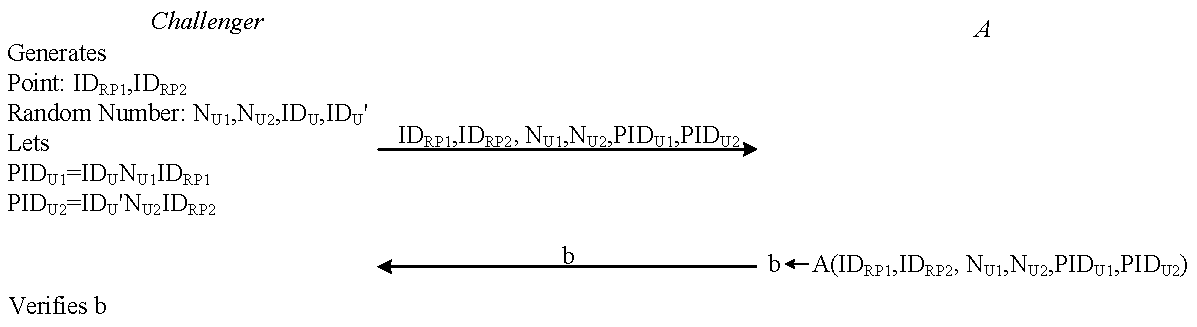
\includegraphics[width=0.82\linewidth]{fig/game1.pdf}
  \caption{The Game.}
  \label{fig:game}
\end{figure*}

\begin{figure*}
  \centering
  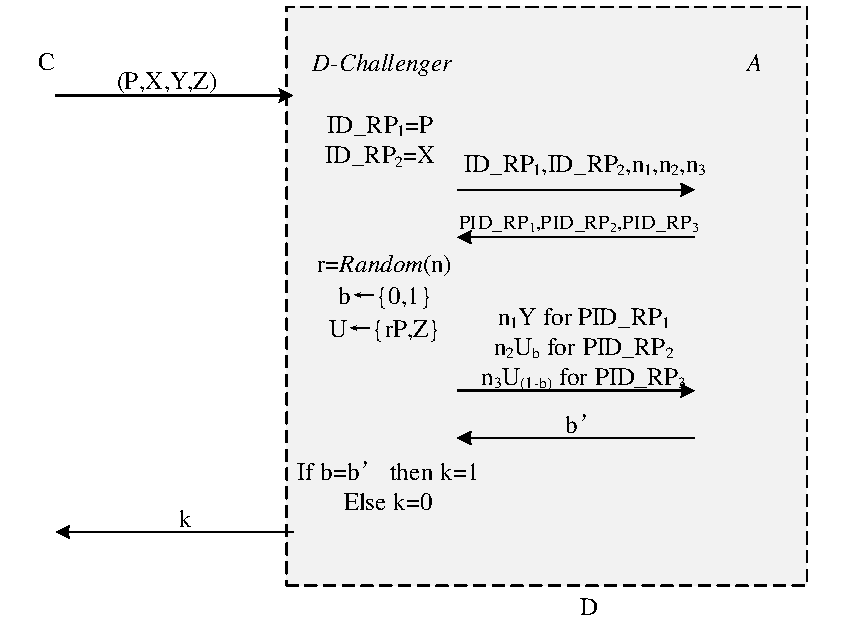
\includegraphics[width=0.65\linewidth]{fig/dalgorithm.pdf}
  \caption{The distinguishing algorithm.}
  \label{fig:dalgorithm}
\end{figure*}

There is the data set, $\langle ID_{RP_j}$, $t_j$, $[ID_U][t_j]{ID_{RP_j}}\rangle$,
    $\langle ID_{RP_{j'}}$, $t_{j'}$, $[ID_{U'}] [t_{j'}] {ID_{RP_{j'}}}\rangle$, from two RPs ($RP_j$ and $RP_{j'}$),
that RP-based identity linkage attack can be considered as these collusive RPs guesses whether $ID_U$ equals $ID_{U'}$.
Here, we can define the game, the adversary owns the same ability as the RP.
The adversary receive the input $\langle ID_{RP_j}$, $t_j$, $[ID_U][t_j]{ID_{RP_j}}\rangle$,
    $\langle ID_{RP_{j'}}$, $t_{j'}$, $[ID_{U'}] [t_{j'}] {ID_{RP_{j'}}}\rangle$, from the challenger, and returns the result $b$.
The $b$ is set 1, when adversary guess that $ID_U$ equals $ID_U'$, otherwise 0.
The game is shown as Figure \ref{fig:game}.
Therefore, whether the RP-based identity linkage attack is possible is equivalent to whether adversary has the advantage on the guessing game.

We define $Pr_1$ is the probability, while the adversary returns $b=1$ as $ID_U$ equals to $ID_U'$.
 And $Pr_2$ is the probability, while the adversary returns $b=1$ but $ID_U$ does not equal to $ID_U'$.
Adversary has the advantage on the game means that
\vspace{-\topsep}
\begin{equation}
Pr_1-Pr_2>\sigma(n)
\end{equation}

While an adversary has the advantage on the guessing game, based on the challenger and adversary,
 we can build a PPT distinguishing algorithm $D$ that breaks DDH assumption.
The algorithm is shown as Figure \ref{fig:dalgorithm}.
That is, the input of $D$ in the form ($X$,$Y$,$Z$,$N$), while $X$,$Y$,$Z$,$N$ are points on the elliptic curve.
The challenger receives the input and set $ID_{RP1}=X$, $ID_{RP2}=Y$, $PID_{U1}=N_{U1} \cdot{Z}$, and $PID_{U2}=N_{U2} \cdot{N}$.  At the end, $D$ returns the $b$ from the adversary as the result.

Now, we let ($P$, $aP$, $bP$, $abP$) and  ($P$, $aP$, $bP$, $cP$) be two inputs.
Thus there is
\vspace{-\topsep}
\begin{multline*}
\ \ \ \ \ \ \ \ \ \ \ \ \ \ \ \ \ Pr[D(P,aP,bP,abP)=1]=\\ Pr[A(P, N_{U1}, b \cdot{N_{U1}P}, aP, N_{U2},b\cdot{N_{U2} aP})=1]=Pr_1\\
Pr[D(P,aP,bP,cP)=1]=\ \ \ \ \ \ \ \ \ \
\\ Pr[A(P, N_{U1}, b \cdot{N_{U1}P}, aP, N_{U2},c/a \cdot{N_{U2}aP})=1]=Pr_2
\end{multline*}
in the first equation $ID_{U} $ and $ ID_{U}'$ all equal to $b$, while in the second equation $ID_{U}$ does not equal to $ID_{U}'$, so that
\begin{equation}
Pr_1-Pr_2=\sigma(n)
\end{equation}
There is a contradiction between equation (4) and equation (5). Therefore, an adversary cannot have the advantage on the guessing game. Thus, the RP-identity linkage attack is computationally impossible.


\begin{figure}[t]
  \centering
  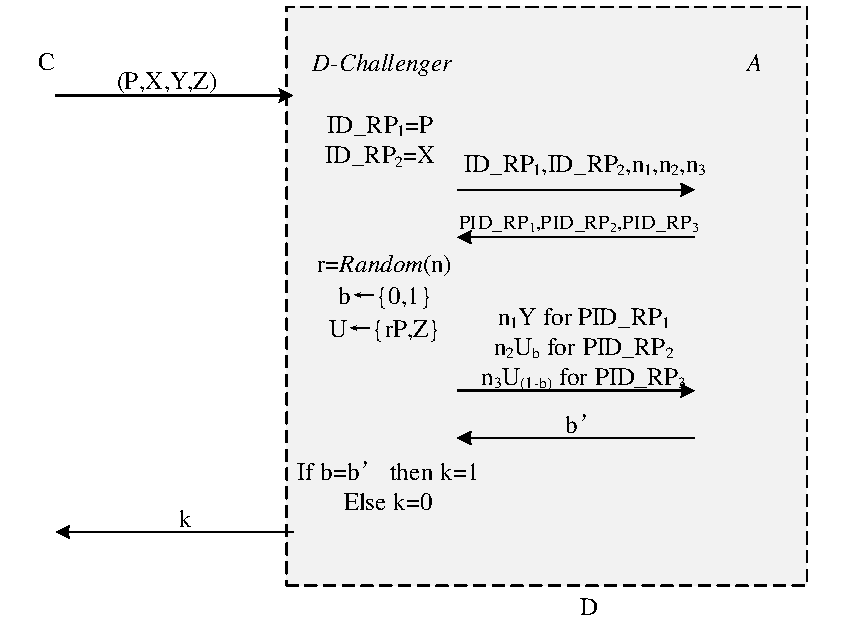
\includegraphics[width=1\linewidth]{fig/dalgorithm.pdf}
  \caption{Distinguishing algorithm.}
  \label{fig:dalgorithm}
\end{figure}
